\documentclass[aps,pre,11pt,a4paper,preprint,amsmath,amssymb,groupedaddress]{revtex4-2}

% latex packages
\usepackage{fix-cm}
\usepackage{bm}
\usepackage{graphicx}
\graphicspath{{figures/}}
\usepackage{xcolor}
\usepackage{booktabs}
\usepackage{listings}
\usepackage{tikz}
\usetikzlibrary{arrows.meta, calc, decorations.pathreplacing}
\usepackage{pgfplots}
\pgfplotsset{compat=1.18}

% times fonts
\usepackage{times}
\usepackage{mathptmx}

% Okabe-Ito colours
\definecolor{oiblack}{HTML}{000000}
\definecolor{oiorange}{HTML}{E69F00}
\definecolor{oisky}{HTML}{56B4E9}
\definecolor{oigreen}{HTML}{009E73}
\definecolor{oiblue}{HTML}{0072B2}
\definecolor{oired}{HTML}{D55E00}
\definecolor{oipurple}{HTML}{CC79A7}
\definecolor{muted}{HTML}{888888}

\lstset{basicstyle=\ttfamily\small, columns=fullflexible, keepspaces=true, frame=single,
        rulecolor=\color{muted}, xleftmargin=1em, xrightmargin=1em, aboveskip=1em, belowskip=1em,
        commentstyle=\color{muted}, language=Python, upquote=true}

% references; cleveref does not resolve all label types under revtex4-2
\newcommand{\Eqref}[1]{Eq.~\eqref{#1}}
\newcommand{\Eqsref}[2]{Eqs.~\eqref{#1} and~\eqref{#2}}
\newcommand{\Figref}[1]{Fig.~\ref{#1}}
\newcommand{\Figsref}[2]{Figs.~\ref{#1} and~\ref{#2}}
\newcommand{\Tabref}[1]{Table~\ref{#1}}
\newcommand{\Secref}[1]{Sec.~\ref{#1}}

% mathematical symbols
\newcommand{\wh}{\widehat}
\newcommand{\ave}[1]{{\left<#1\right>}}
\newcommand{\abs}[1]{{\left|#1\right|}}
\newcommand{\rmd}{\text{d}}
\newcommand{\br}{\ensuremath{\bm{x}}}
\newcommand{\bv}{\ensuremath{\bm{v}}}
\newcommand{\bD}{\ensuremath{\bm{\Delta}}}
\newcommand{\bex}{\ensuremath{\hat{\bm{x}}}}
\newcommand{\bey}{\ensuremath{\hat{\bm{y}}}}
\newcommand{\be}{\ensuremath{\hat{\bm{e}}}}
\newcommand{\T}{\ensuremath{\mathsf{T}}}

% model symbols
\newcommand{\rpsi}{\ensuremath{\rho_\psi}}
\newcommand{\rphi}{\ensuremath{\rho_\varphi}}
\newcommand{\taud}{\ensuremath{\tau_\text{p}}}
\newcommand{\taue}{\ensuremath{\tau_\text{e}}}
\newcommand{\taumax}{\ensuremath{\tau_\text{max}}}
\newcommand{\Wi}{\ensuremath{W^{-1}}}
\newcommand{\w}[1]{\ensuremath{w_{#1}}}
\newcommand{\psh}{\ensuremath{\psi}}
\newcommand{\tlag}{\tau}
\newcommand{\code}[1]{\texttt{#1}}

\begin{document}

\title{Velocity estimation by time delays, the crossing time and full correlation analysis:\\
the model, the methods, their errors on realizations and their implementation in \code{velocity\_estimation}}

\author{J.~M.~Losada and O.~E.~Garcia}
\affiliation{Department of Physics and Technology, UiT The Arctic University of Norway, N-9037 Troms{\o}, Norway}

\date{\today}

\begin{abstract}
This note documents the velocity estimators of the \code{velocity\_estimation} package: time-delay estimation from two and from three points, the crossing time and full correlation analysis (FCA). All are derived for a superposition of uncorrelated pulses that move with a common velocity, have a finite lifetime and are elongated and tilted. The time delays are biased by motion oblique to the separation of the points, by the lifetime and by the tilt of the pulses. The crossing time compares the autocorrelation of a signal with its cross-correlation with a second one at the same lag, which removes any factor of the correlation that depends on the lag alone. FCA adds the zero-lag correlations, which give the shape and tilt of the structures, and from both it gives the velocity vector for any elongation, tilt and lifetime. We describe how the package applies the methods on an imaging grid, how it estimates the correlations from noisy signals and how to call it. Realizations of the process, scanned over the lifetime, the direction of motion, the elongation, the tilt, a spread of velocities and the pixel separation, show the bias and the scatter of each method.
\end{abstract}

\maketitle

%=====================================================================
\section{Introduction}
\label{sec:introduction}

The \code{velocity\_estimation} package estimates a two-dimensional velocity field from a grid of fluctuation measurements, such as gas puff imaging or beam emission spectroscopy arrays, with a few points around each pixel~\cite{losada_three-point_2024}. Its default estimator is time-delay estimation (TDE), which uses the lags that maximize the cross-correlations between the points. This note documents it together with two estimators that use the full correlation functions rather than only the positions of their maxima, and compares them on realizations of a model process.

\emph{Two-point time-delay estimation} (2TDE) divides the distance between two points by the lag that maximizes the cross-correlation of their signals. \emph{Three-point time-delay estimation} (3TDE) combines the delays of two pairs that share a point and are not parallel into a velocity vector~\cite{losada_three-point_2024}. The \emph{crossing time} \taue{} is the lag at which the autocorrelation of one signal equals its cross-correlation with a second signal. Two points a distance $\Delta$ apart then give the velocity component along their separation as $\Delta/2\taue$~\cite{briggs_analysis_1950,woodman_true_1995,holloway_cross_1997}. \emph{Full correlation analysis} (FCA) measures the elongation and tilt of the structures from the correlations at zero lag between three or more points, and corrects the crossing times for them~\cite{phillips_effects_1955,briggs_analysis_1984,armstrong_analysis_1972,holloway_cross_1997a}. Both methods come from spaced-receiver measurements of ionospheric drifts.

In \Secref{sec:model} we define the model, a superposition of pulses, and its cross-correlation function. In \Secref{sec:tde} we derive what the time delays give for it, in \Secref{sec:crossing} the crossing time, in \Secref{sec:shape} the shape from the zero-lag correlations, and in \Secref{sec:fca} the FCA velocity. \Secref{sec:grid} describes how the package applies the estimators around each reference pixel, and \Secref{sec:data} how it estimates the correlations from measured signals. In \Secref{sec:realizations} we compare the four estimators on realizations of the process. \Secref{sec:usage} shows how to call them, and \Secref{sec:limitations} lists the limitations.

%=====================================================================
\section{A superposition of pulses}
\label{sec:model}

Consider a superposition of propagating pulses with a finite lifetime~\cite{pecseli_interpretation_1993,garcia_stochastic_2016},
%
\begin{equation}
\label{eq:process}
\Phi(\br,t) = \sum_{k=1}^{K} a_k\, \psh\big( \br - \bm{\xi}_k - \bv(t-s_k) \big)\, \varphi\!\left( \frac{t-s_k}{\taud} \right).
\end{equation}
%
The sum runs over $K$ uncorrelated pulses, each with an amplitude $a_k$. The pulses have a spatial shape \psh{} and a temporal envelope $\varphi$, which makes each pulse grow and decay over the lifetime \taud. Pulse $k$ is at the position $\bm{\xi}_k$ at the time $s_k$, and all pulses move with the same velocity \bv{} (\Figref{fig:model}a, b).

The cross-correlation function of the process at a separation \bD{} and a lag $\tlag$ is
%
\begin{equation}
\label{eq:ccf_def}
R(\bD, \tlag) = \frac{\ave{\left[ \Phi(\br, t) - \ave{\Phi} \right] \left[ \Phi(\br + \bD, t + \tlag) - \ave{\Phi} \right]}}{\ave{\left[ \Phi(\br, t) - \ave{\Phi} \right]^2}}.
\end{equation}
%
It correlates the point at $\br + \bD$ at the time $t+\tlag$ with the point at \br{} at the time $t$, so that it peaks at a positive lag when the structures move from \br{} towards $\br+\bD$. Campbell's theorem~\cite{rice_mathematical_1944} gives
%
\begin{equation}
\label{eq:ccf_general}
R(\bD, \tlag) = \rpsi\big( \bD - \bv\tlag \big)\, \rphi\!\left( \frac{\tlag}{\taud} \right),
\end{equation}
%
where \rpsi{} and \rphi{} are the normalized autocorrelations of the pulse shape and of its envelope,
%
\begin{equation}
\rpsi(\bm{r}) = \frac{\int \psh(\br)\, \psh(\br + \bm{r})\, \rmd^2x}{\int \psh^2(\br)\, \rmd^2x},
\qquad
\rphi(u) = \frac{\int \varphi(\theta)\, \varphi(\theta + u)\, \rmd\theta}{\int \varphi^2(\theta)\, \rmd\theta}.
\end{equation}
%
At each lag the cross-correlation is the autocorrelation of the pulse shape centred on $\bv\tlag$, and the lifetime lowers it by the factor $\rphi(\tlag/\taud)$, which depends on the lag alone (\Figref{fig:model}c). We call this factor the \emph{decorrelation}.

Elongated and tilted pulses have an elliptic shape, $\rpsi(\bm{r}) = g(\bm{r}^\T \Wi \bm{r})$ with $g$ decreasing and $g(0)=1$. The symmetric, positive-definite matrix
%
\begin{equation}
\label{eq:w}
W = Q_\alpha \begin{pmatrix} \ell_1^2 & 0 \\ 0 & \ell_2^2 \end{pmatrix} Q_\alpha^\T,
\qquad
Q_\alpha = \begin{pmatrix} \cos\alpha & -\sin\alpha \\ \sin\alpha & \cos\alpha \end{pmatrix},
\end{equation}
%
describes structures with the widths $\ell_1 \ge \ell_2$ along their principal axes, the long axis tilted by the angle $\alpha$ from the $x$ axis. Its inverse has the elements
%
\begin{equation}
\label{eq:w_elements}
\w{xx} = \frac{\cos^2\alpha}{\ell_1^2} + \frac{\sin^2\alpha}{\ell_2^2},
\qquad
\w{yy} = \frac{\sin^2\alpha}{\ell_1^2} + \frac{\cos^2\alpha}{\ell_2^2},
\qquad
\w{xy} = \left( \frac{1}{\ell_1^2} - \frac{1}{\ell_2^2} \right) \sin\alpha\cos\alpha,
\end{equation}
%
where we write $\w{ij}$ for $(\Wi)_{ij}$. The off-diagonal element vanishes for round pulses and for pulses aligned with the axes. For Gaussian pulses with a Gaussian envelope, $\psh(\br) \propto \exp(-\br^\T\Wi\br)$ and $\varphi(\theta) \propto e^{-\theta^2}$, the cross-correlation is
%
\begin{equation}
\label{eq:ccf_gauss}
R(\bD, \tlag) = \exp\!\left( - \frac{\tlag^2}{2\taud^2} \right) \exp\!\left[ -\frac{1}{2}(\bD - \bv\tlag)^\T \Wi (\bD - \bv\tlag) \right],
\end{equation}
%
so that $W$ is the covariance of the autocorrelation of the pulse shape. The aim is to estimate \bv{} from $R$ at the handful of separations available around each pixel.

\begin{figure}
\centering
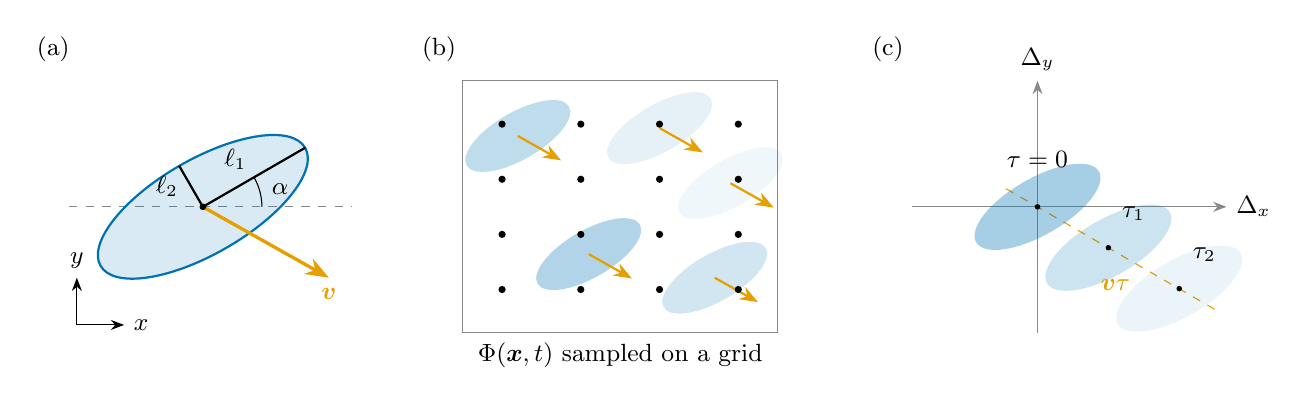
\begin{tikzpicture}[>=Stealth, font=\small]
  % (a) one pulse
  \begin{scope}
    \node at (-1.9, 2.0) {(a)};
    \draw[muted, dashed] (-1.7, 0) -- (1.9, 0);
    \fill[oiblue, fill opacity=0.15, rotate=30] (0,0) ellipse (1.5 and 0.6);
    \draw[oiblue, thick, rotate=30] (0,0) ellipse (1.5 and 0.6);
    \draw[thick, rotate=30] (0,0) -- (1.5,0) node[midway, above left=-1pt] {$\ell_1$};
    \draw[thick, rotate=30] (0,0) -- (0,0.6) node[midway, left=1pt] {$\ell_2$};
    \draw (0.75,0) arc (0:30:0.75); \node at (0.98, 0.22) {$\alpha$};
    \draw[->, very thick, oiorange] (0,0) -- (1.6, -0.9) node[below] {$\bv$};
    \fill (0,0) circle (1.2pt);
    \draw[->] (-1.6,-1.5) -- (-1.0,-1.5) node[right] {$x$};
    \draw[->] (-1.6,-1.5) -- (-1.6,-0.9) node[above] {$y$};
  \end{scope}
  % (b) superposition on a grid of points
  \begin{scope}[xshift=5.3cm]
    \node at (-2.3, 2.0) {(b)};
    \draw[muted] (-2.0,-1.6) rectangle (2.0,1.6);
    \foreach \x/\y/\o in {-1.3/0.9/0.25, 0.5/1.0/0.1, -0.4/-0.6/0.3, 1.2/-0.9/0.18, 1.4/0.3/0.06}{
      \fill[oiblue, fill opacity=\o, rotate around={30:(\x,\y)}] (\x,\y) ellipse (0.75 and 0.3);
      \draw[->, oiorange, thick] (\x,\y) -- ++(0.55,-0.31);
    }
    \foreach \i in {-1.5,-0.5,0.5,1.5}{\foreach \j in {-1.05,-0.35,0.35,1.05}{\fill (\i,\j) circle (1.3pt);}}
    \node[below] at (0,-1.6) {$\Phi(\br,t)$ sampled on a grid};
  \end{scope}
  % (c) the cross-correlation in the plane of separations
  \begin{scope}[xshift=10.6cm]
    \node at (-1.9, 2.0) {(c)};
    \draw[->, muted] (-1.6,0) -- (2.4,0) node[right, black] {$\Delta_x$};
    \draw[->, muted] (0,-1.6) -- (0,1.6) node[above, black] {$\Delta_y$};
    \draw[oiorange, dashed] (-0.4,0.23) -- (2.3,-1.33);
    \foreach \s/\o/\lab in {0/0.35/0, 0.9/0.2/{\tau_1}, 1.8/0.08/{\tau_2}}{
      \fill[oiblue, fill opacity=\o, rotate around={30:(\s,-0.577*\s)}] (\s,-0.577*\s) ellipse (0.9 and 0.36);
      \fill (\s,-0.577*\s) circle (1.0pt);
    }
    \node[above] at (0.0,0.38) {$\tau=0$};
    \node[above right] at (0.95,-0.3) {$\tau_1$};
    \node[above right] at (1.85,-0.82) {$\tau_2$};
    \node[oiorange, below left] at (1.3,-0.8) {$\bv\tau$};
  \end{scope}
\end{tikzpicture}
\caption{(a) An elliptic pulse with the widths $\ell_1$ and $\ell_2$, its long axis tilted by $\alpha$ from the $x$ axis, moving with the velocity \bv. (b) The process: pulses of the same shape and velocity, with amplitudes and lifetimes that make them fade in and out (shading), measured on a grid of points. (c) The cross-correlation $R(\bD,\tlag)$ of \Eqref{eq:ccf_general} in the plane of separations: at each lag it is the autocorrelation of the pulse shape centred on $\bv\tlag$, lowered by the decorrelation $\rphi(\tlag/\taud)$ (shading).}
\label{fig:model}
\end{figure}

%=====================================================================
\section{Time-delay estimation}
\label{sec:tde}

Time-delay estimation uses the lag \taumax{} that maximizes the cross-correlation at a fixed separation. For the Gaussian pulses of \Eqref{eq:ccf_gauss} the logarithm of $R$ is quadratic in the lag, and its maximum is at
%
\begin{equation}
\label{eq:delay}
\taumax(\bD) = \frac{\bD^\T\Wi\bv}{\bv^\T\Wi\bv + 1/\taud^2}.
\end{equation}
%
The delay is linear in the separation. Its denominator holds the two reasons for the cross-correlation to fall with the lag: the pattern moves away, and it decays.

\emph{Two points.} For two points separated by $\bD = \Delta\be$, the 2TDE estimates the velocity component along the separation, $v_\shortparallel = \be\cdot\bv$, as
%
\begin{equation}
\label{eq:2tde}
\wh{v}_\text{2TDE} = \frac{\Delta}{\taumax} = \frac{\bv^\T\Wi\bv + 1/\taud^2}{\be^\T\Wi\bv}.
\end{equation}
%
\emph{Three points.} For a reference point with one point at $\Delta\bex$ and another at $\Delta\bey$, with the delays $\tau_x$ and $\tau_y$, the 3TDE inverts the delays as for a frozen pattern of round pulses, for which $\taumax = \bD\cdot\bv/\abs{\bv}^2$~\cite{losada_three-point_2024},
%
\begin{equation}
\label{eq:3tde}
\wh{\bv}_\text{3TDE} = \frac{\Delta\,(\tau_x, \tau_y)}{\tau_x^2 + \tau_y^2} = \frac{\bv^\T\Wi\bv + 1/\taud^2}{\abs{\Wi\bv}^2}\, \Wi\bv,
\end{equation}
%
where the second equality follows from \Eqref{eq:delay}. Neither estimate depends on the separation $\Delta$. \Eqsref{eq:2tde}{eq:3tde} contain three biases, which we separate by switching on one property of the pulses at a time.

\emph{Misalignment.} For a frozen pattern of round pulses, $\taud = \infty$ and $W = \ell^2 I$, the two estimates are
%
\begin{equation}
\label{eq:misalignment}
\wh{v}_\text{2TDE} = \frac{\abs{\bv}^2}{\be\cdot\bv} = \frac{v_\shortparallel}{\cos^2\beta},
\qquad
\wh{\bv}_\text{3TDE} = \bv,
\end{equation}
%
with $\beta$ the angle between \bv{} and the separation. The 2TDE gives the component along the separation only when the pulses move along it, and it diverges for motion across it. The third point removes this bias.

\emph{Decorrelation.} For round pulses with a finite lifetime,
%
\begin{equation}
\label{eq:decorrelation}
\wh{v}_\text{2TDE} = \frac{v_\shortparallel}{\cos^2\beta} \left( 1 + \frac{\ell^2}{\abs{\bv}^2\taud^2} \right),
\qquad
\wh{\bv}_\text{3TDE} = \bv \left( 1 + \frac{\ell^2}{\abs{\bv}^2\taud^2} \right).
\end{equation}
%
The decorrelation pulls the maximum of the cross-correlation towards shorter lags, so that both estimates are too high, by a factor that is close to one only when a pulse moves much farther than its size within its lifetime, $\abs{\bv}\taud \gg \ell$. The 3TDE keeps the direction. Any factor of the cross-correlation that falls with the lag alone acts in the same way.

\emph{Barber pole.} For a frozen pattern of elongated pulses,
%
\begin{equation}
\label{eq:barberpole}
\wh{v}_\text{2TDE} = \frac{\bv^\T\Wi\bv}{\be^\T\Wi\bv},
\qquad
\wh{\bv}_\text{3TDE} = \frac{\bv^\T\Wi\bv}{\abs{\Wi\bv}^2}\, \Wi\bv.
\end{equation}
%
The 3TDE gives the projection of \bv{} on the direction of $\Wi\bv$, the normal to the contour of the pulse autocorrelation through $\bv$: the estimate is too short and is turned towards the short axis of the pulses, unless \bv{} lies along one of their axes. For pulses moving along $x$, $\bv = v\bex$, the 2TDE of the pair along $x$ gives $v$, and that of the pair along $y$ gives an apparent velocity $v\,\w{xx}/\w{xy}$ across the motion.

%=====================================================================
\section{The crossing time}
\label{sec:crossing}

Take two points a separation \bD{} apart. The crossing time \taue{} is the lag at which the autocorrelation equals the cross-correlation,
%
\begin{equation}
\label{eq:crossing_def}
R(\bm{0}, \taue) = R(\bD, \taue).
\end{equation}
%
Both sides of \Eqref{eq:crossing_def} carry the same decorrelation $\rphi(\taue/\taud)$, which cancels (\Figref{fig:crossing}a). With an elliptic shape what remains is $g\big((\bv\taue)^\T\Wi\bv\taue\big) = g\big((\bD-\bv\taue)^\T\Wi(\bD-\bv\taue)\big)$, and since $g$ is decreasing the two quadratic forms are equal. Expanding them gives the \emph{crossing equation},
%
\begin{equation}
\label{eq:crossing}
\bD^\T \Wi \bv = \frac{\bD^\T \Wi \bD}{2\taue}.
\end{equation}
%
It is linear in \bv{} and holds for any envelope and any elliptic shape. Geometrically, at the crossing time the centre $\bv\taue$ of the correlation is equally far from the two points in the metric of \Wi: it lies on the line through $\bD/2$ normal to $\Wi\bD$, and the contour of $R$ through one point passes through the other (\Figref{fig:crossing}b, c). If $\bD^\T\Wi\bv = 0$ the centre never reaches that line and there is no crossing; \Eqref{eq:crossing} then holds with $1/\taue = 0$.

For round pulses, $W = \ell^2 I$, and with $\bD = \Delta\be$ the crossing equation gives the velocity component along the separation,
%
\begin{equation}
\label{eq:crossing_round}
\wh{v}_\text{e} = \frac{\Delta}{2\taue} = \be\cdot\bv,
\end{equation}
%
exactly, for any lifetime, any direction of motion and any separation. This is the estimator of the method \code{CROSSING} (\Secref{sec:usage}), which computes \Eqref{eq:crossing_round} for each pair. For elongated and tilted pulses, \Eqref{eq:crossing} gives instead
%
\begin{equation}
\label{eq:crossing_barber}
\frac{\Delta}{2\taue} = \frac{\be^\T\Wi\bv}{\be^\T\Wi\be},
\end{equation}
%
which differs from $\be\cdot\bv$ unless \be{} is a principal axis of $W$. Pulses moving along $x$, for example, give a finite crossing time between two points separated along $y$, and so an apparent velocity $v\,\w{xy}/\w{yy}$ along $y$ (\Figref{fig:crossing}c). FCA removes this by measuring \Wi.

\begin{figure}
\centering
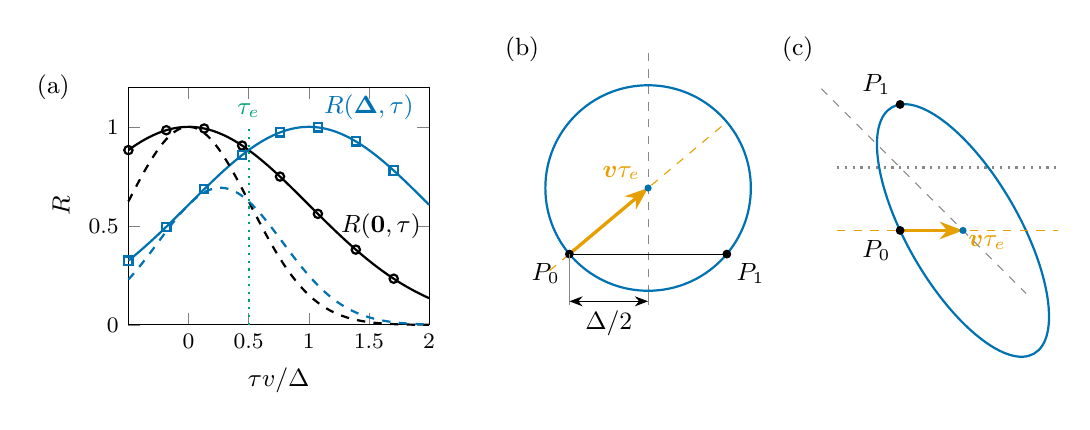
\begin{tikzpicture}[>=Stealth, font=\small]
  % (a) the correlations against the lag
  \begin{axis}[name=ccf, width=5.4cm, height=4.6cm, xmin=-0.5, xmax=2, ymin=0, ymax=1.2,
      xlabel={$\tau v/\Delta$}, ylabel={$R$}, xtick={0,0.5,1,1.5,2}, ytick={0,0.5,1},
      tick label style={font=\footnotesize}, label style={font=\small}, clip=false]
    \node at (rel axis cs:-0.25,1.0) {(a)};
    \addplot[oiblack, thick, domain=-0.5:2, samples=120, mark=o, mark repeat=15, mark size=1.5pt]
      {exp(-x^2/2)};
    \addplot[oiblue, thick, domain=-0.5:2, samples=120, mark=square, mark repeat=15, mark size=1.5pt]
      {exp(-(1-x)^2/2)};
    \addplot[oiblack, thick, dashed, domain=-0.5:2, samples=120] {exp(-x^2/(2*0.6^2))*exp(-x^2/2)};
    \addplot[oiblue, thick, dashed, domain=-0.5:2, samples=120] {exp(-x^2/(2*0.6^2))*exp(-(1-x)^2/2)};
    \draw[oigreen, dotted, thick] (axis cs:0.5,0) -- (axis cs:0.5,1.0);
    \node[oigreen, above] at (axis cs:0.5,1.0) {$\taue$};
    \node[oiblack] at (axis cs:1.6,0.5) {$R(\bm 0,\tau)$};
    \node[oiblue] at (axis cs:1.5,1.1) {$R(\bD,\tau)$};
  \end{axis}
  % (b) round pulses: the bisector
  \begin{scope}[xshift=5.6cm, yshift=0.9cm]
    \node at (-0.6, 2.6) {(b)};
    \draw[muted, dashed] (1,-0.5) -- (1,2.6);
    \draw[oiblue, thick] (1,0.839) circle (1.305);
    \draw[oiorange, dashed] (-0.25,-0.21) -- (2.0,1.678);
    \draw[->, oiorange, very thick] (0,0) -- (1,0.839) node[above left=-1pt] {$\bv\taue$};
    \fill[oiblue] (1,0.839) circle (1.3pt);
    \fill (0,0) circle (1.6pt) node[below left] {$P_0$};
    \fill (2,0) circle (1.6pt) node[below right] {$P_1$};
    \draw[thin] (0,0) -- (2,0);
    \draw[muted, thin] (0,0) -- (0,-0.65) (1,-0.5) -- (1,-0.65);
    \draw[<->, thin] (0,-0.6) -- (1,-0.6) node[midway, below] {$\Delta/2$};
  \end{scope}
  % (c) elongated tilted pulses moving along x, points along y
  \begin{scope}[xshift=9.8cm, yshift=1.2cm]
    \node at (-1.3, 2.3) {(c)};
    \draw[muted, dotted, thick] (-0.8,0.8) -- (2.0,0.8);
    \draw[muted, dashed] (-1.0,1.8) -- (1.6,-0.8);
    \draw[oiblue, thick, rotate around={120:(0.799,0)}] (0.799,0) ellipse (1.806 and 0.71);
    \draw[oiorange, dashed] (-0.8,0) -- (2.0,0);
    \draw[->, oiorange, very thick] (0,0) -- (0.799,0) node[below right=-2pt] {$\bv\taue$};
    \fill[oiblue] (0.799,0) circle (1.3pt);
    \fill (0,0) circle (1.6pt) node[below left] {$P_0$};
    \fill (0,1.6) circle (1.6pt) node[above left] {$P_1$};
  \end{scope}
\end{tikzpicture}
\caption{The crossing time. (a) The autocorrelation (black, circles) and the cross-correlation at $\bD = \Delta\bv/v$ (blue, squares) of round pulses, frozen (solid) and with $\taud = 0.6\,\Delta/v$ (dashed): the decorrelation lowers both but they still cross at $\taue = \Delta/2v$. (b) Round pulses moving obliquely to the separation: at \taue{} the centre of the correlation lies on the perpendicular bisector of the two points (grey dashed), so that its projection on the separation is $\Delta/2$; the contour of $R$ through $P_0$ passes through $P_1$ (blue). (c) Elongated pulses, $\alpha = 120^\circ$, moving along $x$, with the points separated along $y$: the centre never reaches the perpendicular bisector (grey dotted), but it reaches the bisector in the metric of \Wi{} (grey dashed), which gives a crossing time and an apparent velocity along $y$.}
\label{fig:crossing}
\end{figure}

%=====================================================================
\section{The shape from the zero-lag correlations}
\label{sec:shape}

At zero lag the decorrelation is $\rphi(0) = 1$, and for Gaussian pulses \Eqref{eq:ccf_gauss} gives
%
\begin{equation}
\label{eq:shape}
-2\ln R(\bD, 0) = \bD^\T \Wi \bD = \Delta_x^2\, \w{xx} + 2\Delta_x\Delta_y\, \w{xy} + \Delta_y^2\, \w{yy},
\end{equation}
%
one equation, linear in the three elements of \Wi, for each pair of points. Each pair gives the distance, along its separation, from the centre to a contour of $R(\bD,0)$; three separations that are not all parallel fix the ellipse (\Figref{fig:shape}a). For three points at $\bm{0}$, $\Delta\bex$ and $\Delta\bey$, the separations $\Delta\bex$, $\Delta\bey$ and $\Delta(\bey-\bex)$ give
%
\begin{equation}
\label{eq:shape_triangle}
\begin{aligned}
\w{xx} &= -\frac{2\ln R(\Delta\bex, 0)}{\Delta^2},
\qquad
\w{yy} = -\frac{2\ln R(\Delta\bey, 0)}{\Delta^2},
\\
\w{xy} &= \frac{\ln R(\Delta(\bey - \bex), 0) - \ln R(\Delta\bex, 0) - \ln R(\Delta\bey, 0)}{\Delta^2}.
\end{aligned}
\end{equation}
%
With more pairs, \Eqref{eq:shape} is solved by least squares (\Secref{sec:grid}).

The widths and the tilt follow from the eigenvalues and eigenvectors of \Wi,
%
\begin{equation}
\label{eq:shape_parameters}
\frac{1}{\ell_{1,2}^2} = \frac{\w{xx} + \w{yy}}{2} \mp \sqrt{\left(\frac{\w{xx} - \w{yy}}{2}\right)^2 + \w{xy}^2},
\qquad
\alpha = \frac{1}{2}\operatorname{atan2}\!\big(-2\w{xy},\ \w{yy} - \w{xx}\big),
\end{equation}
%
with $\ell_1 \ge \ell_2$ and $\alpha$ in $(-\pi/2, \pi/2]$, the angle of the long axis from the $x$ axis. A measured \Wi{} that is not positive definite has no widths; the package then gives no estimate.

\begin{figure}
\centering
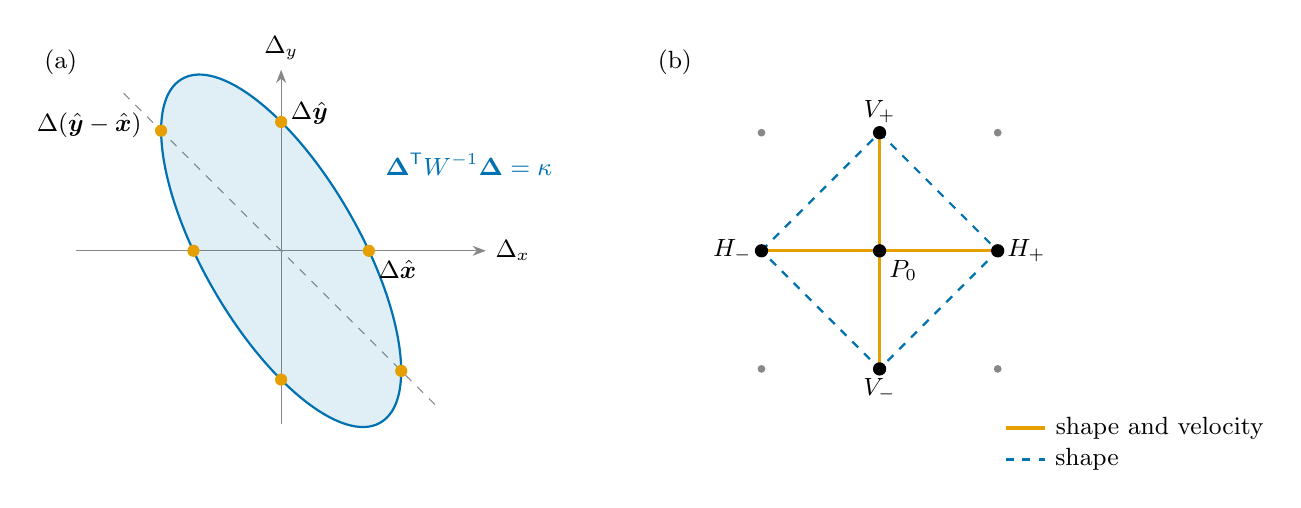
\begin{tikzpicture}[>=Stealth, font=\small]
  % (a) three directions fix the ellipse
  \begin{scope}
    \node at (-2.8, 2.4) {(a)};
    \draw[->, muted] (-2.6,0) -- (2.6,0) node[right, black] {$\Delta_x$};
    \draw[->, muted] (0,-2.2) -- (0,2.3) node[above, black] {$\Delta_y$};
    \draw[muted, dashed] (-2.0,2.0) -- (2.0,-2.0);
    \fill[oiblue, fill opacity=0.12, rotate=120] (0,0) ellipse (2.52 and 0.99);
    \draw[oiblue, thick, rotate=120] (0,0) ellipse (2.52 and 0.99);
    \foreach \x/\y in {1.114/0, 0/1.636, -1.525/1.525}{
      \fill[oiorange] (\x,\y) circle (2.2pt); \fill[oiorange] (-\x,-\y) circle (2.2pt);
    }
    \node[below right] at (1.114,0) {$\Delta\bex$};
    \node[right] at (0,1.75) {$\Delta\bey$};
    \node[left] at (-1.65,1.6) {$\Delta(\bey-\bex)$};
    \node[oiblue, right] at (1.2,1.1) {$\bD^\T\Wi\bD = \kappa$};
  \end{scope}
  % (b) pooled pairs around a reference pixel
  \begin{scope}[xshift=7.6cm]
    \node at (-2.6, 2.4) {(b)};
    \foreach \i in {-1.5,0,1.5}{\foreach \j in {-1.5,0,1.5}{\fill[muted] (\i,\j) circle (1.4pt);}}
    \draw[oiblue, thick, dashed] (-1.5,0) -- (0,1.5) -- (1.5,0) -- (0,-1.5) -- cycle;
    \draw[oiorange, very thick] (-1.5,0) -- (1.5,0);
    \draw[oiorange, very thick] (0,-1.5) -- (0,1.5);
    \fill (0,0) circle (2.4pt) node[below right] {$P_0$};
    \foreach \x/\y/\lab/\pos in {-1.5/0/{H_-}/left, 1.5/0/{H_+}/right, 0/1.5/{V_+}/above, 0/-1.5/{V_-}/below}{
      \fill (\x,\y) circle (2.4pt) node[\pos] {$\lab$};
    }
    \draw[oiorange, very thick] (1.6,-2.25) -- (2.1,-2.25) node[right, black] {shape and velocity};
    \draw[oiblue, thick, dashed] (1.6,-2.65) -- (2.1,-2.65) node[right, black] {shape};
  \end{scope}
\end{tikzpicture}
\caption{(a) The zero-lag correlation at each separation gives, by \Eqref{eq:shape}, the distance from the centre to the contour $\bD^\T\Wi\bD = \kappa$ along that separation (orange dots); three directions, here those of a triangle of points, fix the ellipse. (b) The pairs that the package pools around a reference pixel $P_0$ with its horizontal ($H_\pm$) and vertical ($V_\pm$) neighbours: the four pairs with $P_0$ (orange, solid) enter both the shape and the velocity, and the four diagonal pairs of a horizontal with a vertical neighbour (blue, dashed) enter only the shape.}
\label{fig:shape}
\end{figure}

%=====================================================================
\section{Full correlation analysis}
\label{sec:fca}

FCA solves the crossing equations~\eqref{eq:crossing} with the measured \Wi. Two separations $\bD_1$ and $\bD_2$ that are not parallel give two linear equations for the two components of \bv,
%
\begin{equation}
\label{eq:fca_system}
\begin{pmatrix} \bD_1^\T\Wi \\ \bD_2^\T\Wi \end{pmatrix} \bv
=
\begin{pmatrix} \bD_1^\T\Wi\bD_1 / 2\tau_{\text{e},1} \\ \bD_2^\T\Wi\bD_2 / 2\tau_{\text{e},2} \end{pmatrix}.
\end{equation}
%
For the triangle of \Secref{sec:shape}, with the crossing times $\tau_{\text{e},x}$ and $\tau_{\text{e},y}$ of the pairs separated by $\Delta\bex$ and $\Delta\bey$, the solution is
%
\begin{equation}
\label{eq:fca}
\wh{\bv}_\text{FCA} = W \begin{pmatrix} \w{xx}\, \Delta/2\tau_{\text{e},x} \\ \w{yy}\, \Delta/2\tau_{\text{e},y} \end{pmatrix} = \bv,
\end{equation}
%
exactly, for Gaussian pulses of any elongation, tilt and lifetime, at any separation. The crossing times remove the decorrelation, and the zero-lag shape turns their components back from the metric of \Wi{} to that of the plane. With $\Wi = I$, \Eqref{eq:fca_system} reduces to the crossing time of \Eqref{eq:crossing_round} for each pair. \Tabref{tab:methods} summarizes the four estimators.

\begin{table}
\caption{The four estimators. The time delays need the lag of the maximum of each cross-correlation, the crossing time and FCA the lag at which it meets the autocorrelation; FCA also needs the zero-lag correlations.}
\label{tab:methods}
\begin{ruledtabular}
\begin{tabular}{lp{0.29\textwidth}p{0.2\textwidth}p{0.3\textwidth}}
Method & Uses & Gives & Holds for \\
\colrule
2TDE & \taumax{} of one pair, \Eqref{eq:delay} & $\Delta/\taumax$, \Eqref{eq:2tde} & a frozen pattern moving along the separation \\
3TDE & \taumax{} of two pairs that are not parallel & \bv, \Eqref{eq:3tde} & a frozen pattern of round pulses, any direction of motion \\
\code{CROSSING} & \taue{} per pair, \Eqref{eq:crossing} with $\Wi = I$ & $\be\cdot\bv$ per pair, \Eqref{eq:crossing_round} & round pulses, any lifetime and direction of motion \\
\code{FCA} & $R(\bD,0)$ for \Eqref{eq:shape}, then \taue{} per pair for \Eqref{eq:crossing} & \bv, $\ell_1$, $\ell_2$, $\alpha$ & Gaussian pulses of any elongation, tilt, lifetime and direction of motion \\
\end{tabular}
\end{ruledtabular}
\end{table}

%=====================================================================
\section{On the imaging grid}
\label{sec:grid}

For each reference pixel $P_0$ the package selects its horizontal neighbours $H_\pm$ and vertical neighbours $V_\pm$ (\code{NeighbourOptions}). The time-delay estimates are computed for each of the up to four triangles of $P_0$ with one horizontal and one vertical neighbour, and averaged: the 3TDE from the general form of \Eqref{eq:3tde} for any two separations~\cite{losada_three-point_2024}, and the two-point estimates as the separation over the delay of the horizontal pair for the first component and of the vertical pair for the second. For the crossing time and FCA the package instead collects all the available pairs and solves once (\Figref{fig:shape}b):
%
\begin{itemize}
\item \emph{Shape.} One equation~\eqref{eq:shape} for each pair of $P_0$ with a neighbour, and for each pair of a horizontal with a vertical neighbour: up to eight equations for the three unknowns $\bm{w} = (\w{xx}, \w{xy}, \w{yy})$. Writing them as $A\bm{w} = \bm{b}$, with the rows $(\Delta_x^2, 2\Delta_x\Delta_y, \Delta_y^2)$ of $A$ and $b = -2\ln R(\bD, 0)$, the estimate is the least-squares solution $\wh{\bm{w}} = (A^\T A)^{-1}A^\T\bm{b}$. Pairs of two horizontal or two vertical neighbours, at twice the separation, are left out, since for non-Gaussian pulses $-2\ln R$ there measures a different curvature. Pairs with $R(\bD,0)$ below a minimum (\code{minimum\_correlation}) are also left out.
\item \emph{Velocity.} One crossing equation~\eqref{eq:crossing} for each pair of $P_0$ with a neighbour: up to four equations $M\bv = \bm{c}$ for two unknowns, with the rows $\bD_k^\T\wh{W}^{-1}$ of $M$ and $c_k = \bD_k^\T\wh{W}^{-1}\bD_k/2\tau_{\text{e},k}$. The estimate is the least-squares solution $\wh{\bv} = (M^\T M)^{-1}M^\T\bm{c}$. The method \code{CROSSING} solves the same system with $\wh{W}^{-1} = I$.
\end{itemize}
%
With both diagonals the off-diagonal element comes from two correlations, $\w{xy} = [\ln R(\Delta\bex - \Delta\bey, 0) - \ln R(\Delta\bex + \Delta\bey, 0)]/2\Delta^2$, rather than from three. Opposite neighbours keep the estimate centred on the reference pixel. At a boundary or corner pixel, with a single triangle, the same code solves an exactly determined system. Separations of any length and direction, as on a tilted grid or with \code{max\_separation} above one, need nothing special. Both directions are required: with only horizontal or only vertical neighbours there is no estimate.

%=====================================================================
\section{The correlations from measured signals}
\label{sec:data}

\Figref{fig:data} shows the two steps that turn measured signals into the inputs of \Secref{sec:grid}.

\emph{Normalization without the noise spike.} White measurement noise adds a spike at zero lag to the autocovariance $C(\tlag)$ of each pixel, and to no cross-covariance. Normalizing by the measured variance $C(0)$ would then lower every $R(\bD,0)$ by the factor $1 + \sigma_\text{n}^2/C(0)$, with $\sigma_\text{n}^2$ the noise variance, add a constant to every $-2\ln R$ and bias \Wi; unequal noise at two pixels would also shift their crossing. The package therefore replaces each variance by the autocovariance extrapolated to zero lag from the two smallest nonzero lags. Near zero lag a smooth autocovariance is $C(\tlag) \approx C(0) - a\tlag^2$, and the values at $\rmd t$ and $2\,\rmd t$ give
%
\begin{equation}
\label{eq:spike_free}
C^*(0) = \frac{4C(\rmd t) - C(2\,\rmd t)}{3}
\end{equation}
%
(\Figref{fig:data}a). Every correlation is then normalized as $R_{ab}(\tlag) = C_{ab}(\tlag)/\sqrt{C^*_{aa}(0)\,C^*_{bb}(0)}$. This is on by default (\code{remove\_noise\_spike}) and needs a sampling time well below the correlation time.

\emph{Sign convention.} For the pair of the pixel $P_0$ at $\br_0$ and $P_1$ at $\br_1$, $\bD = \br_1 - \br_0$ and $R(\bD,\tlag)$ correlates $P_1$ at $t + \tlag$ with $P_0$ at $t$, so that it peaks at a positive lag when the structures move from $P_0$ to $P_1$.

\emph{The autocorrelation.} The crossing compares $R(\bD,\tlag)$ with the mean of the two pixels' autocorrelations, $\bar{R}(\tlag) = [R_{00}(\tlag) + R_{11}(\tlag)]/2$. In the model the two are equal. With the mean, swapping the two pixels only changes the sign of \taue, so that a reversed pair is reused from the cache as $R_{10}(\tlag) = R_{01}(-\tlag)$, and an inhomogeneous field, such as the radial profile of the scrape-off layer, does not favour one end of the pair.

\emph{The crossing.} The package looks for the first sign change of $\bar{R}(\tlag) - R(\bD,\tlag)$ on each side of zero lag, within the lag window $[-T, T]$ (\code{window}), refines it on a cubic spline through the samples, and keeps the one nearest zero (\Figref{fig:data}b). Where there is no crossing within the window it takes $1/\taue = 0$, which is the exact value when $\bD^\T\Wi\bv = 0$ (\Secref{sec:crossing}) and otherwise makes an error of at most $\Delta/2T$ in that component. In a record of finite length the difference also changes sign in the tails, where both functions are below their statistical error. The package takes such a sign change as a crossing, at a lag of a few correlation times, and it gives a component of either sign that is small but not negligible against the velocity (\Secref{sec:realizations}).

\emph{Checks and outputs.} A pixel gets no estimate, with a warning, when its separations do not span the plane, when any $R(\bD,0) \le 0$ among the pairs used, or when the fitted \Wi{} is not positive definite. The confidence of an estimate is the smallest maximum of the cross-correlations of the reference pixel with its neighbours. FCA also returns $\ell_1$, $\ell_2$ and $\alpha$ from \Eqref{eq:shape_parameters}.

\begin{figure}
\centering
\begin{tikzpicture}[font=\small]
  % (a) the noise spike and the extrapolation
  \begin{axis}[name=spike, width=7.2cm, height=4.8cm, xmin=-0.05, xmax=1.05, ymin=0.2, ymax=1.5,
      xlabel={$\tau$}, ylabel={$C(\tau)$}, xtick={0,0.2,0.4,0.6,0.8,1.0},
      xticklabels={$0$,$\rmd t$,$2\,\rmd t$,,,}, ytick={0.5,1}, tick label style={font=\footnotesize},
      clip=false]
    \node at (rel axis cs:-0.16,1.06) {(a)};
    \addplot[muted, thin, domain=0:1, samples=80] {exp(-x^2/(2*0.6^2))};
    \addplot[oiblack, only marks, mark=*, mark size=1.8pt] coordinates
      {(0.2,0.9460) (0.4,0.8007) (0.6,0.6065) (0.8,0.4111) (1.0,0.2494)};
    \addplot[oired, only marks, mark=triangle*, mark size=2.6pt] coordinates {(0,1.4)};
    \addplot[oigreen, thick, dashed, domain=0:0.45, samples=40] {0.99430 - (0.9460-0.8007)/(3*0.04)*x^2};
    \addplot[oigreen, only marks, mark=diamond*, mark size=2.8pt] coordinates {(0,0.9943)};
    \node[oired, right] at (axis cs:0.03,1.4) {$C(0)$, with the noise};
    \node[oigreen, right] at (axis cs:0.06,1.07) {$C^*(0)$, \Eqref{eq:spike_free}};
  \end{axis}
  % (b) the sampled crossing
  \begin{axis}[at={(spike.east)}, anchor=west, xshift=1.6cm, width=7.2cm, height=4.8cm,
      xmin=-1.2, xmax=2.0, ymin=0, ymax=1.08, xlabel={$\tau$}, ylabel={$R$},
      xtick={-1,0,1,2}, ytick={0,0.5,1}, tick label style={font=\footnotesize}, clip=false]
    \node at (rel axis cs:-0.16,1.06) {(b)};
    \addplot[oiblack, thin, domain=-1.2:2, samples=100] {exp(-x^2/(2*1.2^2))*exp(-x^2/2)};
    \addplot[oiblue, thin, domain=-1.2:2, samples=100] {exp(-x^2/(2*1.2^2))*exp(-(1-x)^2/2)};
    \addplot[oiblack, only marks, mark=o, mark size=1.8pt, domain=-1.2:2, samples=17]
      {exp(-x^2/(2*1.2^2))*exp(-x^2/2)};
    \addplot[oiblue, only marks, mark=square, mark size=1.8pt, domain=-1.2:2, samples=17]
      {exp(-x^2/(2*1.2^2))*exp(-(1-x)^2/2)};
    \draw[oigreen, dotted, thick] (axis cs:0.5,0) -- (axis cs:0.5,0.84);
    \node[oigreen, right] at (axis cs:0.5,0.1) {$\taue$};
    \node[oiblack, right] at (axis cs:-1.15,0.85) {$\bar{R}(\tau)$};
    \node[oiblue] at (axis cs:1.5,0.97) {$R(\bD,\tau)$};
  \end{axis}
\end{tikzpicture}
\caption{(a) The autocovariance of a pixel, sampled at multiples of $\rmd t$ (black): white noise raises the zero-lag value (red triangle), and \Eqref{eq:spike_free} extrapolates the samples at $\rmd t$ and $2\,\rmd t$ back to zero lag (green dashed line and diamond); the grey line is the noise-free autocovariance. (b) The sampled crossing: the mean autocorrelation (black, circles) and the cross-correlation (blue, squares) are compared on each side of zero lag, and the sign change of their difference, refined on a spline (thin lines), gives \taue; here there is none at negative lags.}
\label{fig:data}
\end{figure}

%=====================================================================
\section{The estimators on realizations}
\label{sec:realizations}

We generate realizations of the process of \Eqref{eq:process} with the \code{blobmodel} package~\cite{losada_blobmodel_2025} and estimate the velocity with the four methods as the package applies them (\Secref{sec:grid}). The pulses are Gaussian with a Gaussian envelope and equal amplitudes, and are recorded on $3\times3$ pixels a distance $\Delta$ apart; the velocity is estimated at the centre pixel. Lengths are given in units of the pulse size $\ell = \sqrt{\ell_1\ell_2}$ and times in units of $\ell/v$, with $v = \abs{\bv}$. Each record lasts $4000\,\ell/v$, sampled every $0.02\,\ell/v$, and all methods use lags up to $8\,\ell/v$. The time delays are the maxima of the cross-correlations on a spline through the samples.

\Tabref{tab:scans} lists the scans. Each varies one property of a base case: a frozen pattern of round pulses that move along $x$, on pixels one pulse size apart. Every case is generated eight times. In the figures the markers give the mean over the eight records and the bars their standard deviation: the distance of a marker from the grey line of no error is the bias of the method, and the bar is the scatter of a single record. The lines give each estimator applied to the model cross-correlation function, \Eqsref{eq:2tde}{eq:3tde} for the time delays and \Eqsref{eq:crossing_barber}{eq:fca} for the crossing time and FCA. Each figure has three panels. Panel (a) shows the two-point estimates of the pair along $x$, the 2TDE and the crossing time, divided by $v_x$. Panels (b) and (c) show the speed and the direction of the three-point estimates: the 3TDE, the crossing times of the pairs along $x$ and $y$ taken as a vector, and FCA.

\begin{table}
\caption{The scans of realizations. Properties that are not listed are those of the base case: a frozen pattern ($\taud = \infty$) of round pulses moving along $x$ ($\beta = 0$) with a single velocity, and $\Delta = \ell$.}
\label{tab:scans}
\begin{ruledtabular}
\begin{tabular}{llll}
Scan & Varied & Other properties & Figure \\
\colrule
Lifetime & $\taud v/\ell$ from $1/2$ to $16$, and $\infty$ & & \ref{fig:scan_lifetime} \\
Direction of motion & $\beta$ from $0$ to $75^\circ$ & & \ref{fig:scan_angle} \\
Elongation & $\ell_1/\ell_2$ from $1$ to $4$ & $\alpha = 30^\circ$ & \ref{fig:scan_aspect} \\
Tilt & $\alpha$ from $0$ to $90^\circ$ & $\ell_1/\ell_2 = 2$ and $4$ & \ref{fig:scan_tilt} \\
Velocity spread & $\sigma_v/v$ from $0$ to $1/2$ & $\taud = 5\ell/v$; round, and $\ell_1/\ell_2 = 2$, $\alpha = 30^\circ$ & \ref{fig:scan_spread} \\
Separation & $\Delta/\ell$ from $0.35$ to $2$ & $\taud = 2\ell/v$, $\ell_1/\ell_2 = 2$, $\alpha = 30^\circ$ & \ref{fig:scan_spacing} \\
Random & all of the above & & \ref{fig:scan_ensemble} \\
\end{tabular}
\end{ruledtabular}
\end{table}

\subsection{Lifetime}

\Figref{fig:scan_lifetime} shows the scan of the lifetime. The time delays overestimate the velocity by the factor of \Eqref{eq:decorrelation}, which grows as the pulses live shorter than the time they take to move their own size. The crossing time and FCA give the speed at every lifetime, since the envelope multiplies the auto- and the cross-correlation alike and drops out of \Eqref{eq:crossing}.

The direction of the crossing time and of FCA scatters more than that of the 3TDE (\Figref{fig:scan_lifetime}c). The pair along $y$ lies across the motion, and its cross-correlation does not cross the autocorrelation. In a record of finite length the difference of the two functions changes sign in the tails, where both are below their statistical error, and the package takes that sign change as a crossing. It gives a component across the motion of either sign, with a mean close to zero. The time delay of the same pair is the maximum of a cross-correlation that peaks at zero lag, and scatters less.

\begin{figure}
\centering
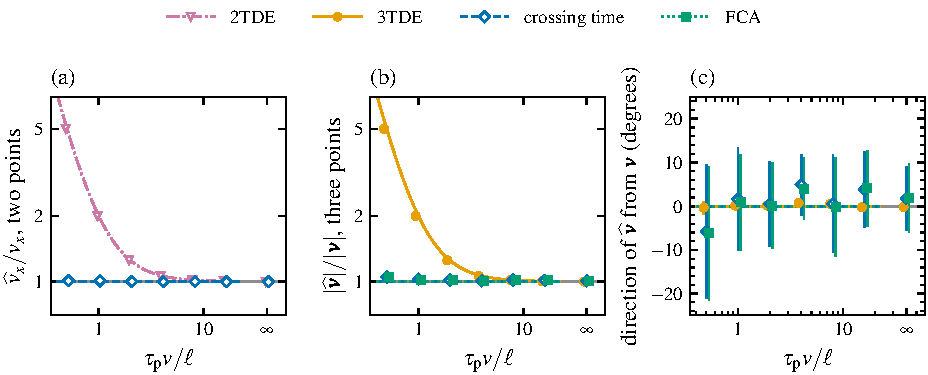
\includegraphics{scan_lifetime}
\caption{Round pulses moving along $x$, against their lifetime; the frozen pattern is at the right end. (a) Two-point estimates of the pair along $x$, (b) speed and (c) direction of the three-point estimates. Markers: mean and standard deviation over eight records. Lines: the estimators on the model correlation function. Grey: no error.}
\label{fig:scan_lifetime}
\end{figure}

\subsection{Direction of motion}

When the velocity makes the angle $\beta$ with the pair, the 2TDE gives the speed of the pattern along the pair, \Eqref{eq:misalignment}, which grows without bound as $\beta$ approaches a right angle (\Figref{fig:scan_angle}a). The crossing time of one pair gives the component $v_x$ for round pulses. The three-point estimates have no bias in the model. In the realizations the crossing time and FCA fall short and scatter in the smaller component at the directions nearest an axis (\Figref{fig:scan_angle}c): the crossing of the pair across the motion lies at a long lag, where the correlations have decayed, and it is found late or not at all.

\begin{figure}
\centering
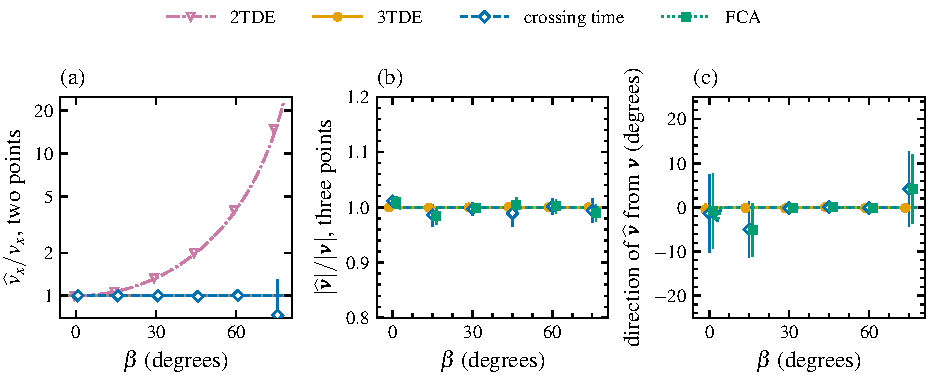
\includegraphics{scan_angle}
\caption{Round frozen pulses, against the angle $\beta$ of their velocity from $x$. Panels and symbols as in \Figref{fig:scan_lifetime}.}
\label{fig:scan_angle}
\end{figure}

\subsection{Elongation and tilt}

\Figsref{fig:scan_aspect}{fig:scan_tilt} show frozen elongated pulses that move along $x$. The pair along $x$ is aligned with the motion, and both two-point estimates give $v_x$. The 3TDE turns towards the short axis of the pulses and gives a lower speed, \Eqref{eq:barberpole}; the error grows with the elongation and is largest at a tilt below $45^\circ$. The crossing-time vector turns the same way, by less at small tilts and by more at large ones, and gives a higher speed, \Eqref{eq:crossing_barber}. FCA gives the velocity at every elongation and tilt. Its scatter is larger where the long axis lies close to a pixel axis, for the reason given for \Figref{fig:scan_lifetime}c.

\begin{figure}
\centering
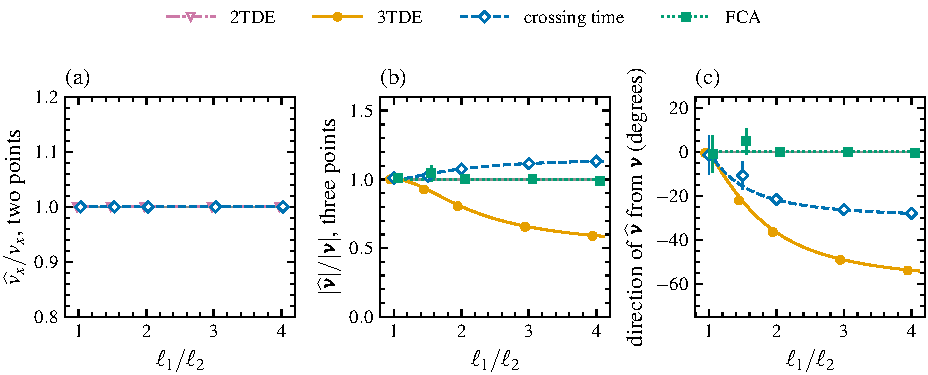
\includegraphics{scan_aspect}
\caption{Frozen pulses moving along $x$ with the long axis at $\alpha = 30^\circ$, against their aspect ratio. Panels and symbols as in \Figref{fig:scan_lifetime}.}
\label{fig:scan_aspect}
\end{figure}

\begin{figure}
\centering
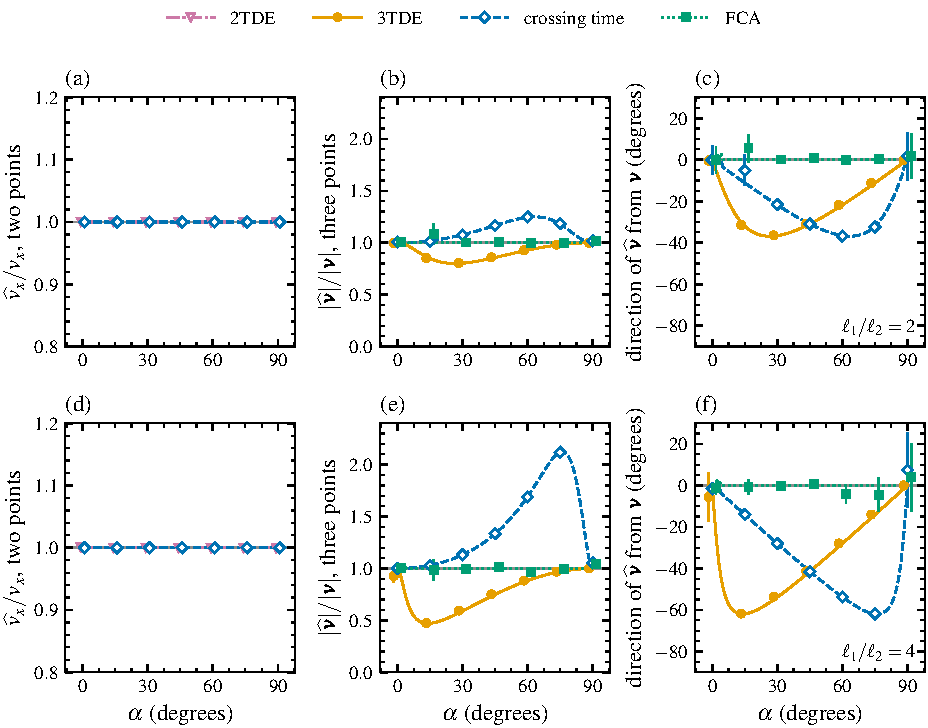
\includegraphics{scan_tilt}
\caption{Frozen pulses moving along $x$, against the tilt $\alpha$ of their long axis, for $\ell_1/\ell_2 = 2$ (top) and $4$ (bottom). Panels and symbols as in \Figref{fig:scan_lifetime}.}
\label{fig:scan_tilt}
\end{figure}

\subsection{A spread of velocities}

None of the estimators models a spread of velocities. Let the velocity of each pulse be normally distributed with mean \bv{} and covariance $\Sigma_V$, independent of where and when the pulse appears. Averaging \Eqref{eq:ccf_gauss} over the velocities gives
%
\begin{equation}
R(\bD,\tlag) = \rho(\tlag)\sqrt{\frac{\det W}{\det W(\tlag)}}\exp\left[-\frac{1}{2}(\bD - \bv\tlag)^\T W(\tlag)^{-1}(\bD - \bv\tlag)\right],
\qquad W(\tlag) = W + \Sigma_V\tlag^2 ,
\label{eq:correlation_spread}
\end{equation}
%
with $\rho(\tlag) = \rphi(\tlag/\taud)$ the decorrelation. The factors in front of the exponential are common to the auto- and the cross-correlation, so that the crossing obeys \Eqref{eq:crossing} with the shape at the crossing lag, $\bD^\T W(\taue)^{-1}(\bD - 2\bv\taue) = 0$. For round pulses with an isotropic spread, $\Sigma_V = \sigma_v^2 I$, $W(\taue)$ is a multiple of the identity and the crossing time gives the mean velocity. Otherwise $W(\taue)$ is rounder than the zero-lag shape that FCA uses, and FCA keeps part of the barber-pole error.

\Figref{fig:scan_spread} shows both cases. The spread adds to the decorrelation, and the time delays overestimate more as it grows. For round pulses the crossing time and FCA give the mean velocity up to the largest spread, half the mean speed. For tilted pulses the FCA error stays small while the spread is small against the mean speed, and grows fast above that, together with its scatter.

\begin{figure}
\centering
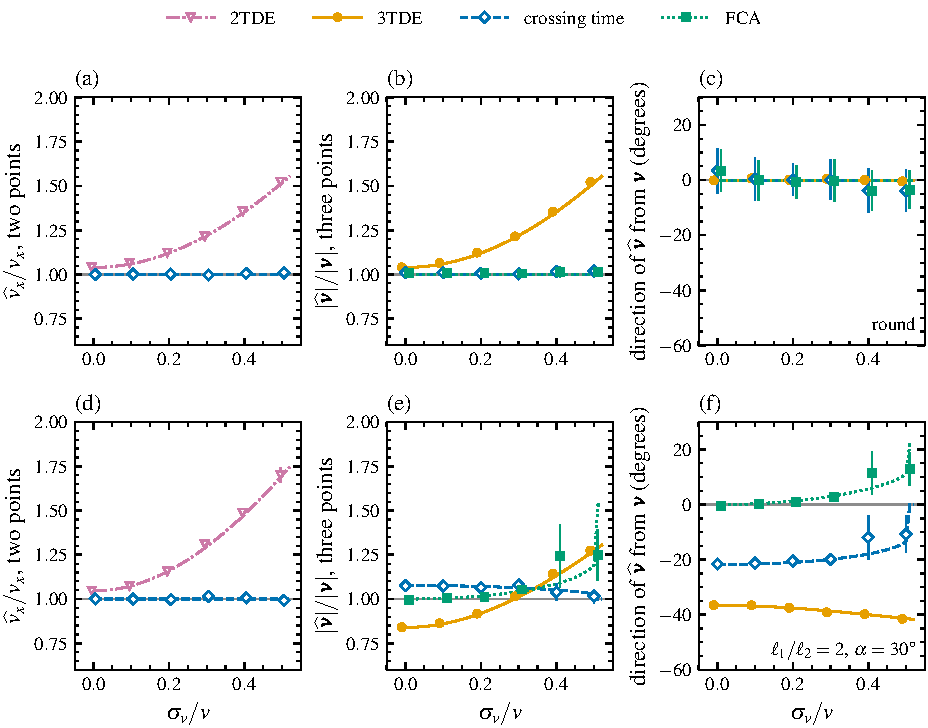
\includegraphics{scan_spread}
\caption{Pulses of lifetime $5\ell/v$ with normally distributed velocities, against the standard deviation $\sigma_v$ of each component: round pulses (top), and $\ell_1/\ell_2 = 2$, $\alpha = 30^\circ$ (bottom). Panels and symbols as in \Figref{fig:scan_lifetime}; the lines use \Eqref{eq:correlation_spread}.}
\label{fig:scan_spread}
\end{figure}

\subsection{Separation}

The biases of the time delays and of the crossing time do not depend on the separation of the pixels (\Figref{fig:scan_spacing}). FCA gives the velocity for separations up to the pulse size. Above it the crossing of the pair along $y$ moves to lags where the correlations have decayed, and the direction scatters. At the largest separation the zero-lag correlation of the diagonal pairs falls below \code{minimum\_correlation}, the fitted shape is not positive definite, and FCA gives no estimate.

\begin{figure}
\centering
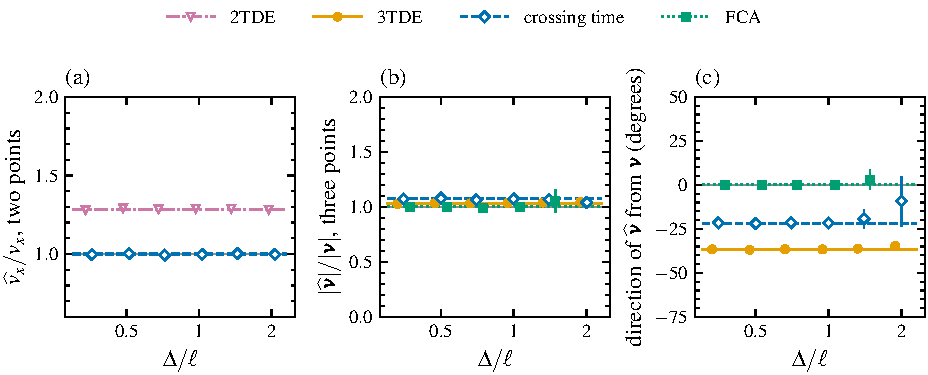
\includegraphics{scan_spacing}
\caption{Pulses with $\taud = 2\ell/v$, $\ell_1/\ell_2 = 2$ and $\alpha = 30^\circ$ moving along $x$, against the pixel separation. Panels and symbols as in \Figref{fig:scan_lifetime}. FCA gives no estimate at the largest separation.}
\label{fig:scan_spacing}
\end{figure}

\subsection{All properties at random}

In the last set every property is drawn at random, one record per case: the lifetime between $\ell/v$ and $16\ell/v$, the aspect ratio between $1$ and $3$, any tilt and any direction of motion, a spread up to $0.3v$, and a separation between $0.5\ell$ and $1.5\ell$. \Figref{fig:scan_ensemble} shows the distribution of the errors over the cases, and \Tabref{tab:ensemble} their median and ninth decile. The errors of the time delays and of the crossing time are those of the model: the thin and the thick lines coincide, so the bias dominates and a longer record would not reduce them. With a tilt and a direction of motion off the pair, the two-point crossing time gives $(\Wi\bv)_x/\w{xx}$ and not $v_x$. FCA has the smallest error; it exceeds the model's because of the scatter of the late crossings, and FCA gives no estimate in a few cases, all at separations near the upper end.

\begin{figure}
\centering
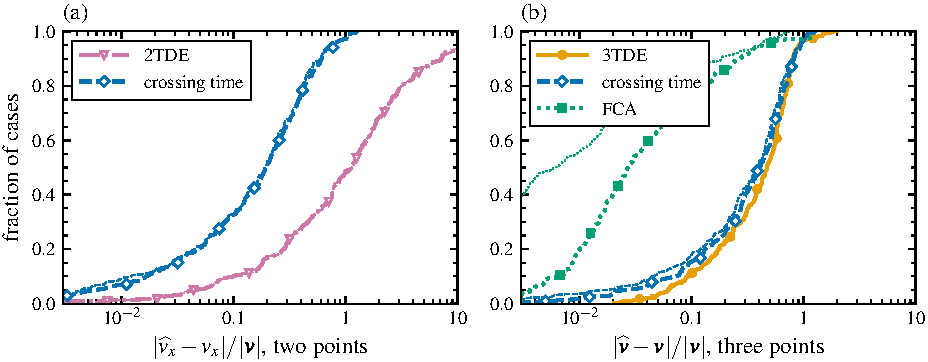
\includegraphics{scan_ensemble}
\caption{Fraction of the random cases with an error below the abscissa: (a) the component along $x$ from two points, (b) the vector from three points. Thick lines with markers: realizations. Thin lines: the estimators on the model correlation function.}
\label{fig:scan_ensemble}
\end{figure}

\begin{table}
\caption{Errors over the random cases, in units of the speed $\abs{\bv}$: $\abs{\wh{v}_x - v_x}$ for the two-point estimates and $\abs{\wh{\bv} - \bv}$ for the three-point ones. A case without an estimate counts as an error above every other.}
\label{tab:ensemble}
\begin{ruledtabular}
\begin{tabular}{llcccc}
& & \multicolumn{2}{c}{Realizations} & \multicolumn{2}{c}{Model} \\
Points & Method & Median & Ninth decile & Median & Ninth decile \\
\colrule
Two & 2TDE & 1.13 & 7.19 & 1.14 & 6.96 \\
Two & Crossing time & 0.19 & 0.62 & 0.19 & 0.60 \\
Three & 3TDE & 0.47 & 0.80 & 0.48 & 0.80 \\
Three & Crossing time & 0.41 & 0.82 & 0.38 & 0.80 \\
Three & FCA & 0.027 & 0.27 & 0.006 & 0.18 \\
\end{tabular}
\end{ruledtabular}
\end{table}

%=====================================================================
\section{Usage}
\label{sec:usage}

The estimator is chosen with the option \code{velocity\_method} of \code{EstimationOptions}, whose default stays time-delay estimation. The crossing time and FCA take their options from \code{FCAOptions}:
%
\begin{lstlisting}
import velocity_estimation.two_dim_velocity_estimates as tdve
from velocity_estimation import utils

eo = tdve.EstimationOptions(
    velocity_method=tdve.VelocityMethod.FCA)
eo.fca_options.window = None   # lag window; None: 100 dt
eo.fca_options.remove_noise_spike = True
eo.fca_options.minimum_correlation = 0.1

data = utils.CModImagingDataInterface(ds)
movie_data = tdve.estimate_velocity_field(data, eo)
vx, vy = movie_data.get_vx(), movie_data.get_vy()
l1, l2 = movie_data.get_l1(), movie_data.get_l2()
tilt = movie_data.get_tilt()
\end{lstlisting}
%
Time-delay estimation uses three points by default, \Eqref{eq:3tde}, and the two-point estimates of \Eqref{eq:2tde} are chosen with \code{use\_3point\_method}; \code{cc\_options} sets how the delays are found. The realizations of \Secref{sec:realizations} use, in the units of that section,
%
\begin{lstlisting}
import velocity_estimation.time_delay_estimation as tde
import velocity_estimation.full_correlation_analysis as fca

cc = tde.CCOptions(cc_window=8, minimum_cc_value=0,
                   interpolate=True)
two = tdve.EstimationOptions(use_3point_method=False,
                             cc_options=cc)
three = tdve.EstimationOptions(cc_options=cc)
full = tdve.EstimationOptions(
    velocity_method=tdve.VelocityMethod.FCA,
    fca_options=fca.FCAOptions(window=8))
\end{lstlisting}
%
and are run and drawn from the repository with \code{python -m fca.scans.run} and \code{python -m fca.scans.figures}.

\code{VelocityMethod.CROSSING} gives the crossing-time velocity of \Eqref{eq:crossing_round} pooled over the pairs, and leaves $\ell_1$, $\ell_2$ and the tilt as NaN. For both methods the options of time-delay estimation (\code{method}, \code{cc\_options}, \code{use\_3point\_method}) are ignored. The tilt is in radians, measured from the first coordinate of the grid.

%=====================================================================
\section{Limitations}
\label{sec:limitations}

\begin{itemize}
\item \Eqref{eq:shape} holds for Gaussian pulses. For other shapes $-2\ln R(\bD,0)$ is not quadratic in \bD, and the fitted \Wi{} depends on the separations used. The crossing equation~\eqref{eq:crossing} holds for any elliptic shape.
\item The noise correction removes white noise only. Coherent pickup and cross-talk between neighbouring channels raise $R(\bD,0)$ and the cross-correlations, and are not corrected.
\item The model has one velocity. With a spread of velocities the shape of the correlation broadens with the lag, \Eqref{eq:correlation_spread}, which the zero-lag shape does not contain. FCA then keeps part of the barber-pole error of elongated, tilted structures, and its scatter grows (\Figref{fig:scan_spread}).
\item A pair across the motion has no crossing, and a pair nearly across it has one at a long lag. In a record of finite length the crossing is then found in the tails of the correlation functions, and the component of the crossing time and of FCA along that pair scatters more than that of the 3TDE (\Figsref{fig:scan_lifetime}{fig:scan_angle}). The same happens at separations above the pulse size (\Figref{fig:scan_spacing}).
\item The extrapolation of \Eqref{eq:spike_free} needs a sampling time well below the correlation time.
\item The shape fit needs separations comparable to the correlation lengths. On a grid much finer than the pulses every $R(\bD,0)$ is close to one, and the error of $\ln R$ is amplified by about $(\ell/\Delta)^2$ in \Wi{} and in the FCA velocity. Spaced-antenna measurements place the sensors at separations where $R(\bD,0)$ is of the order of one half: closer, the FCA speed comes out too small, and farther apart the analysis often fails~\cite{briggs_analysis_1984}. The low speed at small separations, the \emph{triangle size effect}, has been traced to uncorrected noise~\cite{meek_triangle_1990,holdsworth_simple_1995} and to other instrumental errors~\cite{holdsworth_influence_1999}; the normalization of \Secref{sec:data} removes the white-noise part. Larger separations (\code{max\_separation}) condition the fit better, as long as the pairs across the short axis keep $R(\bD,0)$ above \code{minimum\_correlation}. The fit weights all pairs equally and uses the zero lag only; a least-squares fit to the cross-correlations at all lags~\cite{fedor_statistical_1967,baker_estimation_1981} would use more of the data, and is not implemented.
\end{itemize}

\begin{acknowledgments}
This work was supported by the Tromsø Research Foundation through the Trond Mohn Research Foundation's UiT initiative, FUSENOW (TMF2025UiT01).
\end{acknowledgments}

\bibliography{bibliography}

\end{document}
